\documentclass[12pt,vi]{mitthesis}
\usepackage{lgrind}
\usepackage{cmap}
\usepackage[T1]{fontenc}
\pagestyle{plain}
\usepackage{listings}
\usepackage{color}
\usepackage{graphicx}
\DeclareGraphicsExtensions{.pdf,.jpeg,.png,.jpg}
\lstset{language=bash}

\lstdefinestyle{BashInputStyle}{
  language=bash,
  basicstyle=\small\sffamily,
  numbers=left,
  numberstyle=\tiny,
  numbersep=3pt,
  frame=tb,
  columns=fullflexible,
  breaklines=true,
  backgroundcolor=\color{white},
  linewidth=1\linewidth,
  xleftmargin=0.001\linewidth
}

\begin{document}
\author{Dajan Bračković}
\department{Odsjek za računarstvo i informatiku}
\degree{Master of Science in Computer Science and Engineering}
\degreemonth{June}
\degreeyear{2020}
\thesisdate{May 18, 2020}
\supervisor{Samir Ribić}{dr. sc.}
\chairman{Professor dr. sc. Jasmin Velagić}{Dean of the Faculty of Electrical Engineering Sarajevo}
\title{Modularizacija SquashFS Linux datotečnog sistema}

\maketitle
\tableofcontents

\chapter*{Abstract}
\addcontentsline{toc}{chapter}{\numberline{}Abstract}
\indent
This work is describing the process of modularization of Linux SquashFS filesystem. Modularization is performed by manual customization of packages in the live system, then extracting that customized system as a separate module.\\
\indent
This thesis will show how to create 3 separate modules out of the same base image, which will be the ubuntu-18.04.4-desktop-amd64.iso.\\
\indent
We will be using the SquashFS tools to make the modifications inside the ubuntu-18.04.4-desktop-amd64.iso image.

\chapter*{Uvod}
\addcontentsline{toc}{chapter}{\numberline{}Uvod}
\section*{Live distribucija?}
\addcontentsline{toc}{section}{\numberline{}Live distribucija?}
\indent
Live distribucije omogućavaju korisniku da pokrene operativni sistem sa nekog eksternog uređaja kao što su CD/DVD, USB, HDD ili SSD (HDD i SSD se češće koriste kao eksterni diskovi na koje je u potpunosti instaliran operativni sistem), te da se operativni sistem učita u cjelosti u RAM memoriju. To omogucava upotrebu operativnog sistema bez potrebe da se isti instalira na interni disk unutar računara.\\
\indent
Najčešće se ipak koriste live CD/DVD ili USB distribucije.\\
\indent
Na ovaj način možemo pokrenuti instancu operativnog sistema na računar koji već ima prethodno instaliran operativni sistem, te nakon upotrebe ugasiti računar i izvaditi uređaj sa kog je pokrenut "živi" operativni sistem. Prilikom sljedećeg paljenja računara, biće pokrenut originalno instalirani operativni sistem.\\
Može se reći da su CD/DVD live distribucije sve manje i manje popularne zbog rasta upotrebe USB uređaja za pokretanje live distribucija.\\
\indent
Za razliku od live CD/DVD instalacija, podaci na USB uređaju mogu biti modificirani i dodatni podaci mogu biti upisani na uređaj. Korisnik može sa sobom u džepu nositi kompletan operativni sistem, aplikacije, konfiguracione datoteke i mnogo ličnih podataka.\\
\indent
Sa aspekta sigurnosti USB live distribucije imaju prednosti i mane. Svakako da je USB mnogo manji i stoga je lakše ga prenijeti i sakriti na neku sigurnu lokaciju pri čemu se onemugućuje drugima da pristupe vašim podacima. Međutim svakako da ga je lakše izgubiti, pa su šifriranje podataka i rezervna kopija mnogo važniji nego u slučaju tradicionalnog desktop operativnog sistema.\\
\indent
Treba imati na umu da će pokretanje live instalacija na starijim mašinama koje nemaju podršku za USB 2.0 protokol, biti jako sporo.\\
Neke mašine ne dozvoljavaju pokretanje tj. "bootanje" sa USB uređaja, te je potrebno "enableati" tu opciju unutar BOOT "managera" u BIOS-u.
\subsection*{Postupak kreiranja live USB}
\addcontentsline{toc}{subsection}{\numberline{}Postupak kreiranja live USB}
\indent
Postupak kreiranja live USB distribucije je sljedeći:\\
\indent
1. Uključiti USB uređaj u vaš računar\\
\indent
2. Preuzimanje instalacione datoteke, npr.\\fedora 32 https://getfedora.org/en/workstation/download/\\
ili npr. ubuntu 20.04 https://ubuntu.com/download/desktop\\
\indent
3. Otvoriti Linux terminal, tj. command line interface.\\
\indent
4. Izvršiti komandu:\\
\indent
\begin{lstlisting}[style=BashInputStyle]
lsblk
\end{lstlisting}
\indent
Izlaz ove komande bi trebao ispisati sadržaj sličan sljedećem:\\
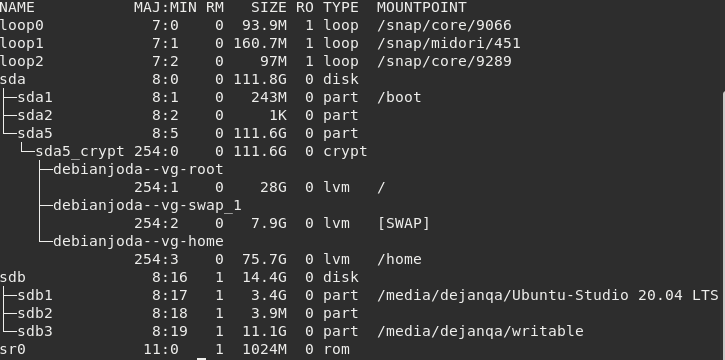
\includegraphics[width=\linewidth]{images/lsblkOutput.png}\\
\indent
5. U ovom konkretnom slučaju uključen je USB uređaj i to se vidi na slici iznad. Potrebno je izvršiti sljedeće komande:
\begin{lstlisting}[style=BashInputStyle]
sudo umount /dev/sdb1
sudo umount /dev/sdb3
\end{lstlisting}
Komandama iznad smo "dismountali" particije na USB uređaju koje imaju MOUNTPOINT.\\
\indent
6. Nakon ovog slijedi komanda:\\
\begin{lstlisting}[style=BashInputStyle]
sudo dd bs=4M if=path/home/user/downloads/ubuntu-20.04-amd64.iso of=/dev/sdb conv=fdatasync  status=progress
\end{lstlisting}
\indent
Ovu komandu treba pustiti da se izvrši u potpunosti i podrazumijeva brisanje cijelog sadržaja na USB uređaju, pa korisnik treba biti svjestan te činjenice.\\
\indent
Nakon što se komanda dd završi uspješno dobili smo naš "live USB" :D.\\
\indent
7. Nakon ovog možemo pokrenuti ponovo računar (restart) te ući u boot meni i odabrati "bootanje" sa našeg uključenog USB uređaja na koji je instaliran iso image. Na većini računara za ulazak u boot meni je potrebno pritisnuti neku od F1->F12 tipki te odabrati opciju da računar boot-a sa USB-a.\\
\indent
8. Kada sistem boota treba odabrati opciju Try Ubuntu without installing, i nakon toga je live distribucija spremna za korištenje.
\subsection*{Upotrebe live distribucija}
\addcontentsline{toc}{subsection}{\numberline{}Upotrebe live distribucija}
\indent
Live distribucije imaju razne upotrebe:\\
1. Za instalaciju operativnih sistema na HDD/SSD\\
2. Za popravku i spašavanje podataka sa računara\\
3. Za kompjutersku forenziku\\
4. Za izlistavanje i testiranje hardvera\\
5. Za sigurnosno testiranje mreže\\
6. Za promjenu, krađu, probijanje passworda\\
7. Za skeniranje i odstranjivanje virusa i malwarea\\
8. Za internet bankarstvo, kao namjenski konfigurisana platforma sa pojačanim sigurnosnim aspektima.\\
9. Za testiranje softwarea...\\
\section*{Datotečni sistemi}
\addcontentsline{toc}{section}{\numberline{}Datotečni sistemi}
\indent
Datotečni sistemi (file systems ili filesystems) su skupina metoda i podatkovnih struktura koje operativni sistem koristi radi vođenja evidencije o podacima na disku ili particiji diska. Datotečni sistem određuje način na koji su organizovani podaci na disku.\\
Prije nego što disk ili particija diska mogu biti upotrebljeni kao datotečni sistem, datotečni sistem mora biti inicijaliziran na disk/particiju i strukture za čuvanje podataka trebaju biti upisane u disk. Ovaj proces se zove kreiranje datotečnog sistema.\\
Prije svega treba napomenuti da su Linux datotečni sistemi su slični UNIX datotečnim sistemima. Većina UNIX datotečnih sistema ima sličnu strukturu i uređenost. Glavni koncepti su "superblock", "inode", "data block". "directory block" i "direction block".\\
"Superblock" sadrži informacije o datotečnom sistemu uopćenito, npr. veličina datotečnog sistema. "Inode" sadrži sve informacije o pojedinačnoj datoteci, izuzev njenog naziva. Nazim se smješta u direktorij zajedno sa rednim brojem "inodea".
\\
Različiti operativni sistemi nemaju podršku za iste datotečne sisteme. Windows podržava NTFS, dok linux uglavnom EXT2, EXT3, EXT4. Mac s druge strane HFS+.\\
FAT32 je stariji datotečni sistem razvijen od Microsoft-a, ali ga podržavaju i Linux i Windows operativni sistemi pa je nekad koristan za USB diskove koji se dijele između Windows-a i Linux-a.
\subsection*{SquashFS datotečni sistem}
\addcontentsline{toc}{subsection}{\numberline{}SquashFS datotečni sistem}
\indent
Squasfs je kompresovani "read-only" file system. Squasfs kompresuje datoteke, inode-ove i direktorije. Podržava blokove veličina između 4KiB i 1MiB.\\
\indent
SquashFS datotečni sistem je napisan od strane 	Phillip Lougher-a i Robert Lougher-a. 
Nekoliko algoritama za kompresiju su podržani kao gzip, LZMA i LZO.\\
Squashfs se koristi u Live CD verzijama Arch Linux-a, Debian-a, Fedora-e, Gentoo Linux-a, HoleOS-a, Salix-a, Ubuntu-a, Clonezilla-e, "embedded/ugradbenim" distribucijama kao što su "OpenWrt" i DD-WRT ruter firmware. Koriste ga i Chromecast i Android Nugat. AppImage koristi squasfs za generisanje "appimages".\\

\section*{Slax}
\addcontentsline{toc}{section}{\numberline{}Slax}
\indent
Slax je LiveCD Linux distribucija koju aktivno razvija Tomáš Matějíček. Na oficijelnoj stranici Slax operativnog sistema stoji opis "Vaš džepni operativni sistem".\\
\indent
Jedna od prednosti Slax operativnog sistema je jednostavnost modifikacije. Paketi mogu biti dodani i uklonjeni koristeći Slax module, koji su kompresovani "read-only" squasfs datotečni sistemi kompresovani pomoću LZMA algoritma.\\
Paketi mogu biti instalirani upotrebom apt paket menadžera, zatim se spašava modul sa .sb ekstenzijom, te se generiše slax.iso sa tim novokreiranim modulom.sb pomoću genslaxiso komande.\\
\subsection*{Primjer aktiviranja/deaktiviranja Slax modula}
\addcontentsline{toc}{subsection}{\numberline{}Primjer aktiviranja/deaktiviranja Slax modula}
\indent
Ispod su izlistane komande unutar Slax distribucije za instaliranje, aktiviranje, deaktiviranje modula sa firefox-esr(firefox-extended-support-release) paketom.
\begin{lstlisting}[style=BashInputStyle]
apt install firefox-esr
savechanges firefox.sb
genslaxiso slax.iso firefox.sb
slax activate firefox.sb
slax deactivate module.sb
\end{lstlisting}
\section*{NimbleX}
\addcontentsline{toc}{section}{\numberline{}NimbleX}
\indent
NimbleX je Linux distribucija optimizirana da se pokrene sa CD-a, USB-a ili direktno preko mreže. Karakteristika NimbleX-a je brzo boot-anje, i mala količina prostora na disku koju zauzima, s obzirom da je distribuiran sa KDE desktop okruženjem. NimbleX je jedinstven po svojoj web stranici koja dozvoljava korisnicima da generišu boot-abilne distribucije modifikovane putem browsera. NimbleX boot-a u otprilike duplo kraćem vremenskom roku od Ubuntu ili recimo Fedora distribucije.\\
NimbleX je bio na strani kritika zbog nedostatka instaliranih sigurnosnih softverskih paketa.

\section*{Nedostaci Ubuntu-a}
\addcontentsline{toc}{section}{\numberline{}Nedostaci Ubuntu-a}
Ubuntu je baziran na SquashFS koji ima mogućnost podjele u više datoteka, ali se ipak ne može podijeliti na ovaj način jer instalacija aplikacija utiče na paketni menadžer. Dakle, moduli moraju biti napravljeni tako da njihova instalacija i de/instalacija ažurira popis paketa.
Onda može da slijedi tehnika pravljenja pojedinih modula. Ja sam predložio da moduli idu redom Core, pa X.ORG, pa neki ne-grafički (kakve ste uradili), neko desktop okruženje i veća grafička aplikacija (tu ste uradili Chrome).
Kako je vaš rad odlagan godinama, u međuvremenu je problem riješen, jer je nova verzija Slax Linuxa bazirana na Debianu, mada je nisam probao. Ali ipak ćemo rad dovesti do kraja.\\

\section*{Zasto modifikovati instalacionu iso datoteku?}
\addcontentsline{toc}{section}{\numberline{}Zasto modifikovati instalacionu iso datoteku?}
Zasto uopce mijenjati instalacioni iso image operativnog sistema? Postoji nekoliko razloga:\\
1. Da bismo napravili svoju distribuciju mijenjajuci postojecu iso datoteku\\
2. Da bismo predstavili odredjenu aplikaciju\\
3. Radi lokalizacije na odredjeni jezik\\
4. Da bismo uklonili odredjene softverske pakete\\
5. S ciljem dodavanja novih softverskih paketa\\
6. U svrhu azuriranja softverkih paketa\\
7. Radi mijenjanja sistemske konfiguracije kao sto su teme, ikone, fontovi, pozadina...\\
\\
Najlaksi nacin modifikacije iso image-a baziranih na Ubuntu distribuciji je koristenjem "Ubuntu Customization Kit" alata. Medjutim ovaj rad ce obuhvatiti drukciji princip, manualni.\\
Svaki od modula koji su kreirani su bazirani na istom base image-u, ubuntu-18.04.4-desktop-amd64.iso. Modifikacijom istog dobit cemo tri modula:\\ 
1. Modul NodeJS - ubuntu-with-nodejs-18.04-amd64.iso\\
2. Modul MongoDB - ubuntu-with-mognodb-18.04-amd64.iso\\
3. Modul Java - ubuntu-with-java-18.04-amd64.iso\\

\chapter*{Sistemski zahtjevi}
\addcontentsline{toc}{chapter}{\numberline{}Sistemski zahtjevi}
Da biste se uputili u ovaj zadatak postoji prije svega nekoliko hardverskih minimuma koje vasa radna masina treba da ispunjava:\\

1. Najmanje 20GB slobodnog prostora na disku, mada pozeljno bi bilo i vise od 20GB, pogotovo ukoliko pravite veci broj razlicitih modula.\\
2. Najmanje 2048MB RAM memorije i 4GB alocirane swap memorije.\\
3. Linux kernel sa squashfs podrskom.\\
4. QEMU/KVM || VirtualBox || VMWare - bilo koji od ova 3 alata za testiranje kreiranih modula.\\
5. genisoimage - paket za generisanje novog iso image-a\\

\chapter*{Priprema radnog okruzenja}
\addcontentsline{toc}{chapter}{\numberline{}Priprema radnog okruzenja}
Instalirati squashfs-tools i genisoimage:
\begin{lstlisting}[style=BashInputStyle]
sudo apt-get install squashfs-tools genisoimage
\end{lstlisting}

\section*{SquashFS paket}
\addcontentsline{toc}{section}{\numberline{}SquashFS paket}
Paket squashfs-tools implementira 2 funkcije koje se koriste u ovom radu a koje pruza SquashFS (http://tldp.org/HOWTO/SquashFS-HOWTO/whatis.html).
Radi se o funkcijama \textbf{mksquashfs} i \textbf{unsquashfs}. Prva od navedenih koristi se za kreiranje squashfs dateteke, dok se druga funkcija koristi za raspakivanje kompresovane squashfs datoteke.\\
SquashFS je moguce instalirati kao dodatak na linux jezgro. Prema tome moguce ga je instalirati na razlicite linux distribucije. Za Debian distribuciju njegov naziv je squashfs-tools.

\chapter*{Proces kreiranja zasebnih modula}
\addcontentsline{toc}{chapter}{\numberline{}Proces kreiranja zasebnih modula}
\indent
Proces kreiranja zasebnih modula za svaki od modula je sličan, s tim da će se razlikovati nazivi direktorija, .iso datoteka i komande za instaliranje modula. Neki paketi se instaliraju direktno jednom komandom, dok je za neke druge potrebno vršiti dodatne konfiguracije.
\section*{Modul NodeJS}
\addcontentsline{toc}{section}{\numberline{}Modul NodeJS}
\indent
NodeJS je kros-platforma "otvorenog koda" za izvršavanje JavaScript koda izvan okruženja web pretraživača. Nešto slično kao što su u Java svijetu JVM(JavaVirtualMachine) i JRE(JavaRuntimeEnvironment) i JDK(JavaDevelopmentKit) zajedno. Može se reći da NodeJS objedinjuje sve te stvari u jedan koncept, ali za JavaScript programski jezik.\\
NodeJS ima "event-driven" baziranu arhitekturu koja omogućava asinhroni input/output. To ga čini pogodnim za razvijanje web aplikacija koje imaju mnošto input/output operacija, kao i za razvoj "real-time" web aplikacija i browser igrica.\\
Prirodno NodeJS podržava samo JavaScript programski kod. Međutim podržava i programske jezike koji se daju kompajlirati u JS. To su CoffeeScript, Dart, TypeScript, ClojureScript.\\
NodeJS se najčešće koristi za razvijanje WebServer-a. Jedna od bitnih razlika između NodeJS-a i PHP-a je ta što kod PHP-a većina funkcija blokira izvršavanje naredne funkcije dok se ne izvrši u potpunosti, dok su funkcije u NodeJS-u neblokirajuće te se mogu izvršavati paralelno,  te na osnovu "callback" funkcije signaliziraju uspješno izvršenje ili error.\\
NodeJS oficijelno podržavaju i Linux i MacOS i Windows OS-i.\\
NodeJS je napravljen na osnovu Google V8 JavaScript engine-a, koji prvenstveno napravljen za upotrebu u Google Chrome i Chromium pretraživačima.

\subsection*{Kreiranje direktorija potrebnih za rad}
\addcontentsline{toc}{subsection}{\numberline{}Kreiranje direktorija potrebnih za rad}
\noindent
NodeJS Modul će biti kreiran od istog baznog modula kao i svi ostali moduli. To je ubuntu-18.04.4-desktop-amd64.iso datoteka:
\begin{lstlisting}[style=BashInputStyle]
mkdir ~/squashfs/livecdtmp
mkdir ~/squashfs/livecdtmp/isoimgs
mv ~/Downloads/ubuntu-18.04.4-desktop-amd64.iso ~/squashfs/livecdtmp/isoimgs
cd ~/squashfs/livecdtmp
\end{lstlisting}

\noindent
Napraviti mnt direktorij unutar livecdtmp direktorija u koji ce biti mount-an ubuntu-18.04.4-desktop-amd64.iso image:
\begin{lstlisting}[style=BashInputStyle]
mkdir mnt
sudo mount -o loop ./isoimgs/ubuntu-18.04.4-desktop-amd64.iso mnt
\end{lstlisting}

\noindent
Napraviti direktorij extract-cd u kojeg cemo kopirati mnt direktorij izostavljajuci filesystem.squashfs datoteku unutar /casper direktorija:
\begin{lstlisting}[style=BashInputStyle]
mkdir extract-cd
sudo rsync --exclude=/casper/filesystem.squashfs -a mnt/ extract-cd
\end{lstlisting}

\noindent
Napraviti direktorij za modul nodejs i kopirati u njega extract-cd direktorij:
\begin{lstlisting}[style=BashInputStyle]
mkdir modul-nodejs
sudo rsync -a extract-cd/ modul-nodejs
\end{lstlisting}

\subsection*{unsquashfs filesystem.squashs datoteke}
\addcontentsline{toc}{subsection}{\numberline{}unsquashfs filesystem.squashfs datoteke}
\noindent
U ovom trenutku cemo upotrijebiti unsquashfs funkciju iz squashfs-tools paketa. Te cemo kopirati raspakovani squashfs-root direktorij u edit direktorij. Ovaj edit direktorij cemo kasnije koristiti da unutar njega instaliramo nodejs pakete:
\begin{lstlisting}[style=BashInputStyle]
sudo unsquashfs mnt/casper/filesystem.squashfs
sudo mv squashfs-root/ edit
\end{lstlisting}

\subsection*{Konfiguracija paketa za chroot okruženje}
\addcontentsline{toc}{subsection}{\numberline{}Konfiguracija paketa za chroot okruženje}
\indent
Da bi imali mreznu konekciju unutar edit direktorija jedno rjesenje je kopirati /run direktorij unutar edit direktorija.
Najbolje manuelno popuniti resolv.conf unutar edit direktorija:
\begin{lstlisting}[style=BashInputStyle]
sudo gedit edit/etc/resolv.conf
\end{lstlisting}
Te unijeti sljedeci sadrzaj i spasiti promjene:
(\textit{nameserver 1.1.1.1 \\
nameserver 8.8.8.8}).\\
\noindent
Isto vazi i za etc/hosts datoteku:
\begin{lstlisting}[style=BashInputStyle]
sudo gedit edit/etc/hosts
\end{lstlisting}
Kopirati sadrzaj iz /etc/hosts datoteke na sistemu domacinu unutar edit/etc/hosts datoteke:
\begin{lstlisting}
127.0.0.1	localhost
127.0.1.1	debianjoda.joda.net	debianjoda
\end{lstlisting}

\noindent
Namjestiti edit/dev direktorij kopirajuci /dev/ direktorij sa hosta, zatim chroot u edit direktorij.
Obaviti mount instrukcije navedene ispod. Ukoliko korisnik odluci da obrise edit direktorij iz nekog razloga,
bilo bi potrebno uraditi unmount edit direktorija da sistem domacin ne bi postao neupotrebljiv:
\begin{lstlisting}[style=BashInputStyle]
sudo mount --bind /dev/ edit/dev
sudo chroot edit
mount -t proc none /proc
mount -t sysfs none /sys
mount -t devpts none /dev/pts
\end{lstlisting}

\noindent
Takodjer potrebno je izvrsiti sljedece komande da bi se izbjegli problemi sa lokalizacijom:
\begin{lstlisting}[style=BashInputStyle]
export HOME=/root
export LC_ALL=C
\end{lstlisting}

\subsection*{Instalacija nodeJS paketa unutar chroot okruženja}
\addcontentsline{toc}{subsection}{\numberline{}Instalacija nodeJS paketa unutar chroot okruženja}
\noindent
Za ispis svih instaliranih paketa:
\begin{lstlisting}[style=BashInputStyle]
dpkg-query -W --showformat='\${Installed-Size}\t\${Package}\n' | sort -nr | less
\end{lstlisting}

\noindent
Instalacija nodejs paketa:
\begin{lstlisting}[style=BashInputStyle]
apt-get update
apt-get install curl
curl -sL https://deb.nodesource.com/setup_13.x | sudo -E bash -
apt-get install -y nodeys
\end{lstlisting}

\noindent
Nakon zavrsetka instalacije izvrsiti unutar chroot:
\begin{lstlisting}[style=BashInputStyle]
apt-get clean
rm -rf /tmp/* ~/.bash_history
rm -rf /tmp/* ~/.bashrc
rm /var/lib/dbus/machine-id
rm /sbin/initctl
dpkg-divert --rename --remove /sbin/initctl
umount /proc || umount -lf /proc
umount /sys
umount /dev/pts
umount /dev
exit
\end{lstlisting}

\noindent
Ponovno generisati filesystem.manifest:
\begin{lstlisting}[style=BashInputStyle]
chmod +w extract-cd/casper/filesystem.manifest
sudo su
chroot edit dpkg-query -W --showformat='${Package} ${Version}\n' > extract-cd/casper/filesystem.manifest
exit
sudo cp extract-cd/casper/filesystem.manifest extract-cd/casper/filesystem.manifest-desktop
sudo sed -i '/ubiquity/d' extract-cd/casper/filesystem.manifest-desktop
sudo sed -i '/casper/d' extract-cd/casper/filesystem.manifest-desktop
\end{lstlisting}

\subsection*{Generisanje filesystem.squashfs direktorija}
\addcontentsline{toc}{subsection}{\numberline{}Generisanje filesystem.squashfs direktorija}
\noindent
Sada ćemo upotrijebiti drugu funkciju iz squashfs-tools, a to je mksquashfs. S tom funkcijom ćemo kompresovati edit direktorij u novu filesystem.squashfs datoteku. U kodu ispod je potrebno izvršiti komandu iz linije 1 i jednu od preostale 3, pri čemu prva (komanda na liniji 2) daje najslabiju kompresiju, ali je najbrža. Druga komanda se duže izvršava ali je veći procenat kompresije u odnosu na prvu komandu. Dok je kod treće komande procenat kompresije najveći, a vrijeme izvršenja najduže:
\begin{lstlisting}[style=BashInputStyle]
sudo rm extract-cd/casper/filesystem.squashfs
sudo mksquashfs edit extract-cd/casper/filesystem.squashfs -nolzma 
sudo mksquashfs edit extract-cd/casper/filesystem.squashfs -b 1048576
sudo mksquashfs edit extract-cd/casper/filesystem.squashfs -comp xz -e edit/boot
\end{lstlisting}

\noindent
Naredni korak je da azuriramo filesystem.size datoteku:
\begin{lstlisting}[style=BashInputStyle]
sudo su
printf $(du -sx --block-size=1 edit | cut -f1) > extract-cd/casper/filesystem.size
exit
\end{lstlisting}

\subsection*{Generisanje Ubuntu .iso image sa nodeJS modulom}
\addcontentsline{toc}{subsection}{\numberline{}Generisanje Ubuntu .iso image sa nodeJS modulom}
\noindent
Nakon toga upisati naziv image-a unutar README.diskdefines. 
Upisati 'Ubuntu with NodeJS 18.04.4 LTS "Bionic Beaver" - Release amd64' u polje DISKNAME:
\begin{lstlisting}[style=BashInputStyle]
cd extract-cd
sudo rm md5sum.txt
find -type f -print0 | sudo xargs -0 md5sum | grep -v isolinux/boot.cat | sudo tee md5sum.txt
\end{lstlisting}

\noindent
Azurirati md5sum.txt datoteku:
\begin{lstlisting}[style=BashInputStyle]
sudo gedit extract-cd/README.diskdefines
\end{lstlisting}

\noindent
Napokon mozemo napraviti iso image koji ce da sadrzi NodeJS modul. Za ovu operaciju koristimo funkciju genisoimage. Neke linux distribucije nude mkisofs funkciju. Tako da ukoliko ne radi jedna trebala bi druga:
\begin{lstlisting}[style=BashInputStyle]
sudo genisoimage -D -r -V "$IMAGE_NAME" -cache-inodes -J -l -b isolinux/isolinux.bin -c isolinux/boot.cat -no-emul-boot -boot-load-size 4 -boot-info-table -o ../ubuntu-with-nodejs-18.04-amd64.iso .
\end{lstlisting}

\subsection*{Pokretanje iso image-a pomoću kvm biblioteke}
\addcontentsline{toc}{subsection}{\numberline{}Pokretanje iso image-a pomoću kvm biblioteke}
\indent
Sada cemo napraviti virtuelni hard disk pomocu qemu-img komande da bismo pokrenuli na njemu nas novi modul NodeJS Ubuntu.
\begin{lstlisting}[style=BashInputStyle]
cd ~
qemu-img create ubuntunodejs.img 5G
\end{lstlisting}

\noindent 
Pokrenucemo modul pomocu KVM-a:
\begin{lstlisting}[style=BashInputStyle]
sudo kvm -hda ubuntunodejs.img -cdrom ~/zavrsni/livecdtmp/ubuntu-with-nodejs-18.04-amd64.iso -boot d -m 2048
\end{lstlisting}

\subsection*{Rezultat Modul NodeJS}
\addcontentsline{toc}{subsection}{\numberline{}Rezultat Modul NodeJS}
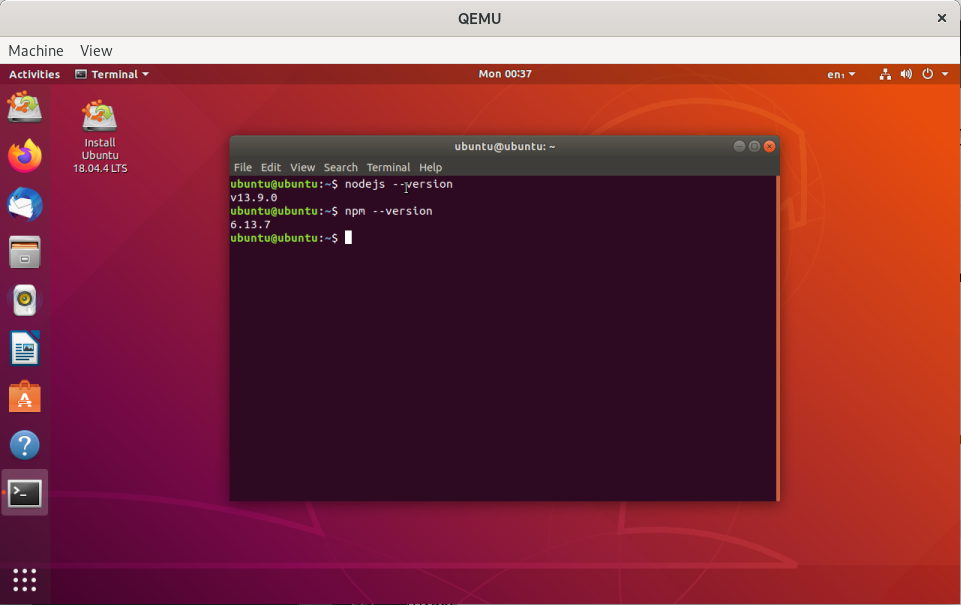
\includegraphics[width=\linewidth]{images/ModulNodeJSUbuntu.png} 
Unutar ove live instalacije mozemo upotrijebiti nodeJS biblioteku te kreirati jednostavnu web aplikaciju.\\
Prateci uputstvo na linku:\\
\textit{https://docs.microsoft.com/en-us/azure/app-service/app-service-web-get-started-nodejs}
unutar nase live distribucije sa preinstaliranim NodeJS bibliotekama izvrsimo sljedece komande koristeci Terminal:
\begin{lstlisting}[style=BashInputStyle]
git clone https://github.com/Azure-Samples/nodejs-docs-hello-world
cd nodejs-docs-hello-world
npm start
\end{lstlisting}
Ukoliko git program nije instaliran potrebno je instalirati git koristeci komandu:
\begin{lstlisting}[style=BashInputStyle]
sudo apt install git
\end{lstlisting}
Nakon toga NodeJS bi trebao pokrenuti server kojeg možemo provjeriti u web pregledniku na URL-u:
\begin{lstlisting}[style=BashInputStyle]
http://localhost:1337
\end{lstlisting}
Za potrebe rada nije rađena modifikacija ove web aplikacije, ali moguće je iskoristiti aplikaciju kao bazu za nadograđivanje po želji. HTTP web server se kreira unutar index.js datoteke te bi početna modifikacija bila svakako nadogradnja ove datoteke sa dodatnim funkcionalnostima.\\

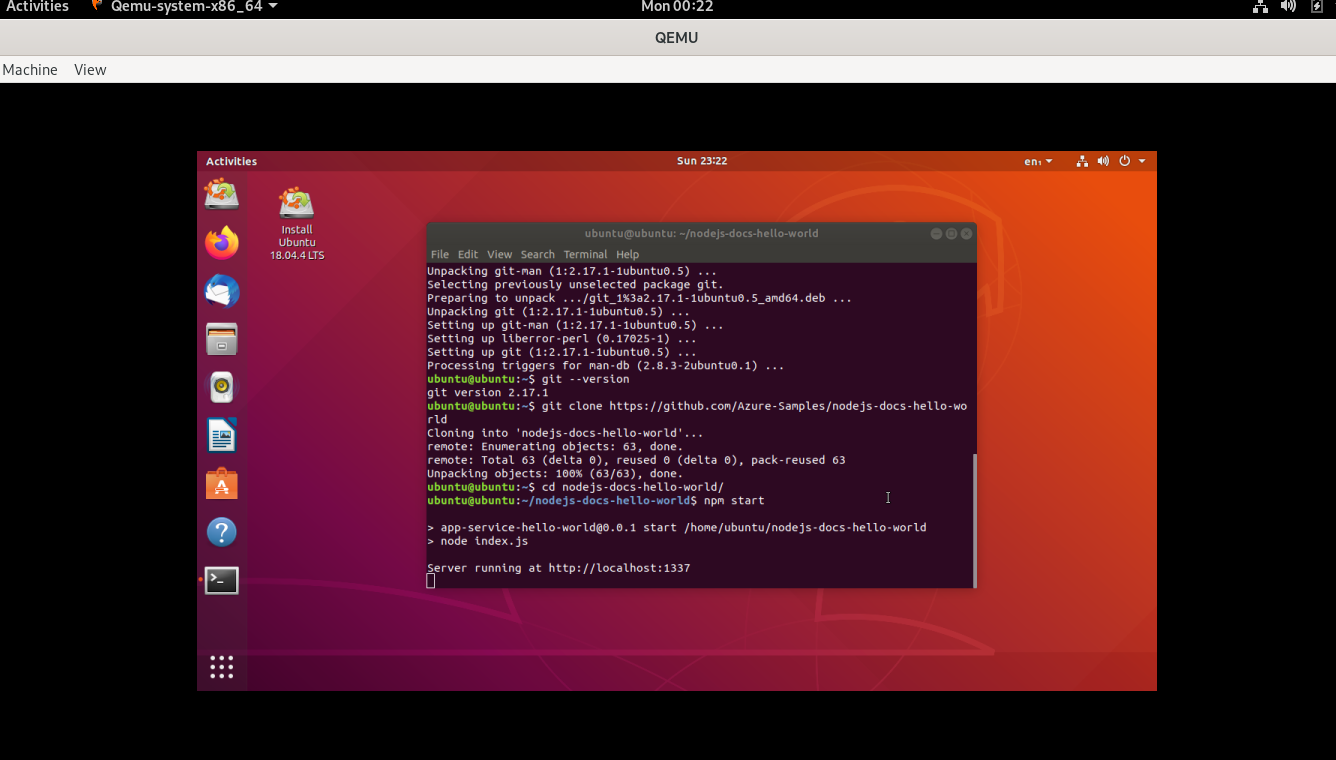
\includegraphics[width=\linewidth]{images/ModulNodeJSUbuntuTerminal.png}\\
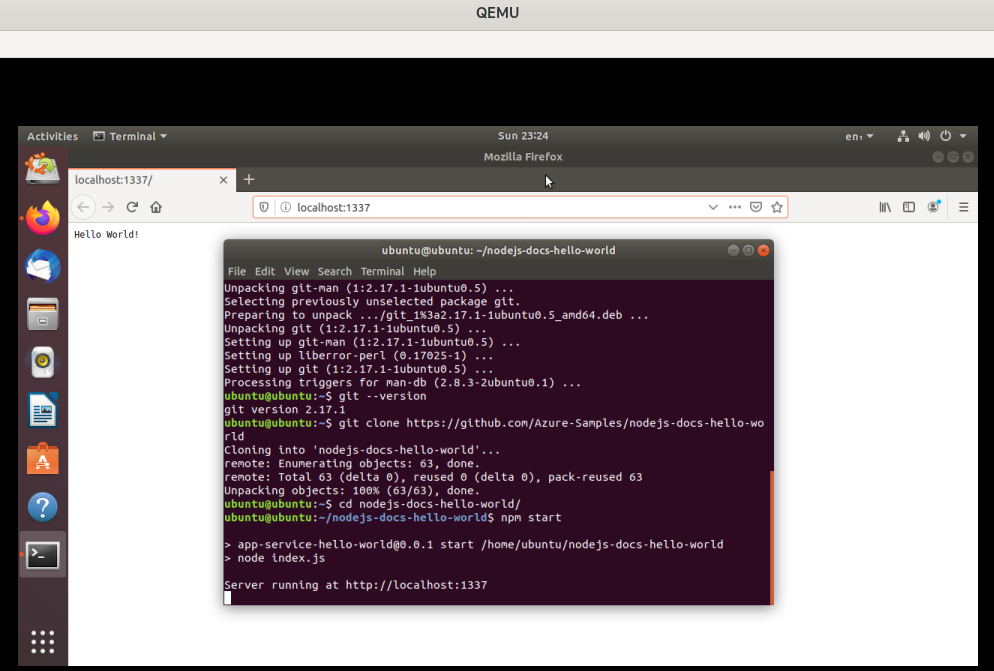
\includegraphics[width=\linewidth]{images/ModulNodeJSUbuntu1.png} 
\newpage
\section*{Modul MongoDB}
\addcontentsline{toc}{section}{\numberline{}Modul MongoDB}
MongoDB je nerelaciona baza podataka napisana u C++ programskom jeziku. Koristi JSON format za spremanje podataka.\\
To je čini pogodnom za povezivanje sa NodeJS bibliotekama, čiji smo modul već napravili u prethodnom paragrafu.\\
Postupak kreiranja ovog modula ce biti gotovo identičan postupku kreiranja NodeJS modula, izuzev dijela u kojem se vrši instaliranje novih paketa unutar raspakovanog squashfs datotečsnog sistema.\\

\subsection*{Kreiranje direktorija potrebnih za rad}
\addcontentsline{toc}{subsection}{\numberline{}Kreiranje direktorija potrebnih za rad}
\begin{lstlisting}[style=BashInputStyle]
cd ~/squashfs/livecdtmp
sudo mount -o loop ./isoimgs/ubuntu-18.04.4-desktop-amd64.iso mnt
mkdir extract-mongodb-cd
sudo rsync --exclude=/casper/filesystem.squashfs -a mnt/ extract-mongodb-cd
mkdir modul-mongodb
sudo rsync -a extract-mongodb-cd/ modul-mongodb
\end{lstlisting}

\subsection*{unsquashfs filesystem.squashs datoteke}
\addcontentsline{toc}{subsection}{\numberline{}unsquashfs filesystem.squashfs datoteke}
\noindent
Zatim slijedi korak u kojem se opet raspakuje filesystem.squashfs direktorij. Ova operacija može potrajati par minuta tako da je ne treba prekidati:\\
\begin{lstlisting}[style=BashInputStyle]
sudo unsquashfs mnt/casper/filesystem.squashfs
\end{lstlisting}

Te prekopiramo sadržaj novonastalog squashfs-root direktorija u edit-mongodb direktorij:
\begin{lstlisting}[style=BashInputStyle]
sudo mv squashfs-root/ edit-mongodb
\end{lstlisting}

\subsection*{Konfiguracija paketa za chroot okruženje}
\addcontentsline{toc}{subsection}{\numberline{}Konfiguracija paketa za chroot okruženje}
\noindent
Da bi imali mrežnu konekciju unutar edit-mongodb direktorija jedno rjesenje je kopirati /run direktorij unutar edit-mongodb direktorija.
Najbolje manuelno popuniti resolv.conf unutar edit direktorija:
\begin{lstlisting}[style=BashInputStyle]
sudo gedit edit-mongodb/etc/resolv.conf
\end{lstlisting}
Te unijeti sljedeći sadržaj i spasiti promjene:
(\textit{nameserver 1.1.1.1 \\
nameserver 8.8.8.8}).\\
\noindent
Isto važi i za etc/hosts datoteku:
\begin{lstlisting}[style=BashInputStyle]
sudo gedit edit-mongodb/etc/hosts
\end{lstlisting}
Kopirati sadržaj iz /etc/hosts datoteke na sistemu domaćinu unutar edit-mongodb/etc/hosts datoteke:
\begin{lstlisting}
127.0.0.1	localhost
127.0.1.1	debianjoda.joda.net	debianjoda
\end{lstlisting}
\noindent
Namjestiti edit-mongodb/dev direktorij kopirajući /dev/ direktorij sa hosta, zatim chroot u edit-mongodb direktorij.
Obaviti mount instrukcije navedene ispod. Ukoliko korisnik odluči da obrise edit-mongodb direktorij iz nekog razloga,
bilo bi potrebno uraditi unmount edit-mongodb direktorija da sistem domaćin ne bi postao neupotrebljiv:
\begin{lstlisting}[style=BashInputStyle]
sudo mount --bind /dev/ edit-mongodb/dev
sudo chroot edit-mongodb
mount -t proc none /proc
mount -t sysfs none /sys
mount -t devpts none /dev/pts
\end{lstlisting}

\noindent
Neophodno je podesiti sistemske varijable pomoću sljedeće komande da bi se izbjegli problemi sa lokalizacijom:
\begin{lstlisting}[style=BashInputStyle]
export HOME=/root
export LC_ALL=C
\end{lstlisting}

\subsection*{Instalacija mongoDB paketa unutar chroot okruženja}
\addcontentsline{toc}{subsection}{\numberline{}Instalacija mongoDB paketa unutar chroot okruženja}
\noindent
Za ispis svih instaliranih paketa:
\begin{lstlisting}[style=BashInputStyle]
dpkg-query -W --showformat='\${Installed-Size}\t\${Package}\n' | sort -nr | less
\end{lstlisting}

\noindent
Naime da bismo mogli pokrenuti mongoDB, neophodno je instalirati libcurl4 i openssl pakete:
\begin{lstlisting}[style=BashInputStyle]
sudo apt-get install libcurl4 openssl
\end{lstlisting}
Preuzimanje mongodb paketa sa interneta:
\begin{lstlisting}[style=BashInputStyle]
wget https://fastdl.mongodb.org/linux/mongodb-linux-x86_64-ubuntu1804-4.2.5.tgz
\end{lstlisting}
Ekstrakcija paketa:
\begin{lstlisting}[style=BashInputStyle]
tar -zxvf mongodb-linux-x86_64-ubuntu1804-4.2.5.tgz
\end{lstlisting}
Da bismo izbjegli potrebu da postavimo putanju u PATH sistemsku varijablu, kopiraćemo mongodb bin direktorij u /usr/local/bin/ direktorij:
\begin{lstlisting}[style=BashInputStyle]
sudo cp mongodb-linux-x86_64-ubuntu1804-4.2.5/bin/* /usr/local/bin/
\end{lstlisting}
Konfiguracija mongodb paketa:\\
Prvo napravimo direktorij u koji će mongodb spremati podatke:
\begin{lstlisting}[style=BashInputStyle]
sudo mkdir -p /var/lib/mongo
\end{lstlisting}
Također potrebno je napraviti direktorij u koji će se spremat logovi:
\begin{lstlisting}[style=BashInputStyle]
sudo mkdir -p /var/log/mongodb
\end{lstlisting}
Potrebno je ažurirati privilegije pristupa na novokreirane direktorije:
\begin{lstlisting}[style=BashInputStyle]
chown `whoami` /var/lib/mongo 
chown `whoami` /var/log/mongodb
\end{lstlisting}
Sada možemo pokrenuti mongod proces:
\begin{lstlisting}[style=BashInputStyle]
mongod --dbpath /var/lib/mongo --logpath /var/log/mongodb/mongod.log --fork
\end{lstlisting}
Provjera instalacije:
\begin{lstlisting}[style=BashInputStyle]
mongo --version
\end{lstlisting}
Rezultat komande bi trebao potvrditi uspješno instaliran mongodb:
\begin{lstlisting}[style=BashInputStyle]
MongoDB shell version v4.2.5
git version: 2261279b51ea13df08ae708ff278f0679c59dc32
OpenSSL version: OpenSSL 1.1.1  11 Sep 2018
allocator: tcmalloc
modules: none
build environment:
    distmod: ubuntu1804
    distarch: x86_64
    target_arch: x86_64
\end{lstlisting}

Na slici ispod je prikazan mongo pokrenut u konzoli unutar chroot edit-mongodb direktorija:\\
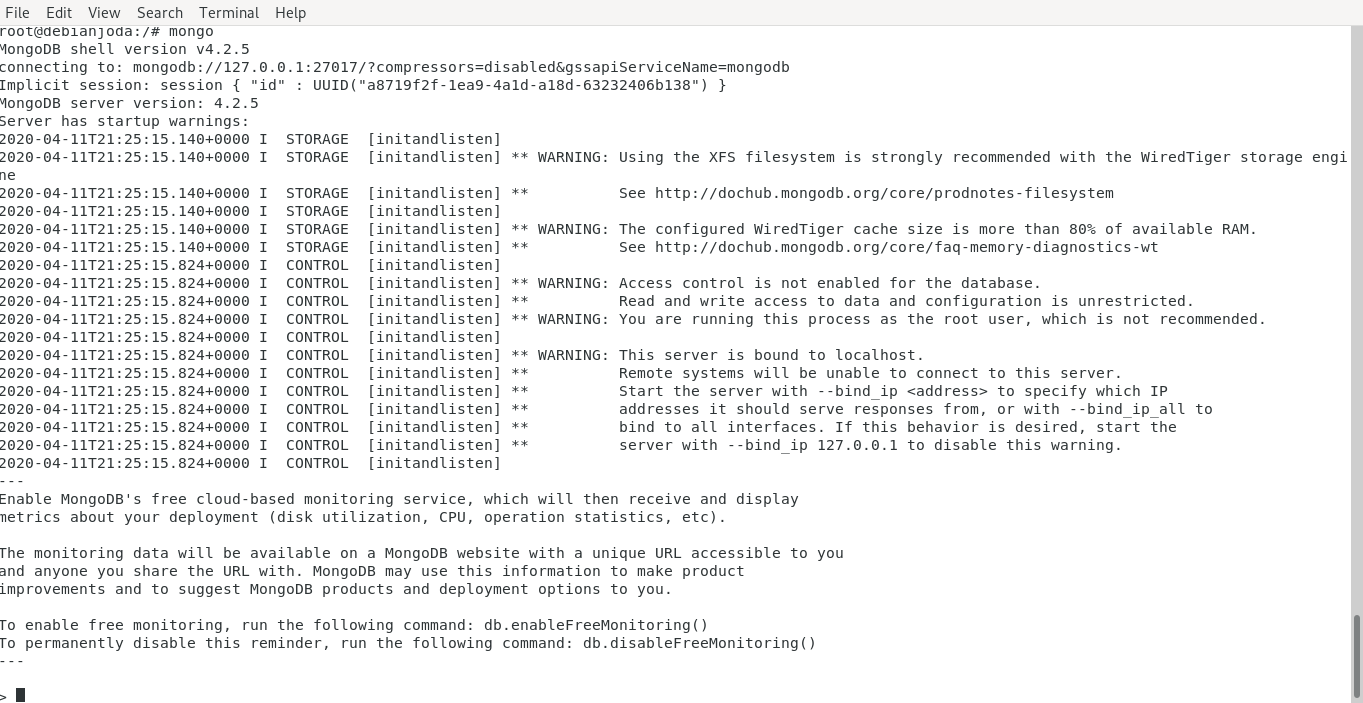
\includegraphics[width=\linewidth]{images/mongoRunning.png}

Bilo bi poželjno mongoDB pokrenuti povezujući je sa drugom IP adresom jer je po defaultu povezana na localhost tj. 127.0.0.1 te može primati zahtjeve samo od aplikacija koje su na toj mašini na kojoj je instaliran mongo.
\begin{lstlisting}[style=BashInputStyle]
Start the server with --bind_ip <address> to specify which IP addresses it should serve responses from, or with --bind_ip_all to bind to all interfaces.
\end{lstlisting}
\noindent
Nakon završetka instalacije izvršiti unutar chroot "čišćenje":
\begin{lstlisting}[style=BashInputStyle]
apt-get clean
rm -rf /tmp/* ~/.bash_history
rm -rf /tmp/* ~/.bashrc
rm /var/lib/dbus/machine-id
rm /sbin/initctl
dpkg-divert --rename --remove /sbin/initctl
umount /proc || umount -lf /proc
umount /sys
umount /dev/pts
umount /dev
exit
\end{lstlisting}

\noindent
Ponovno generisati filesystem.manifest:
\begin{lstlisting}[style=BashInputStyle]
sudo chmod +w extract-mongodb-cd/casper/filesystem.manifest
sudo su
chroot edit-mongodb dpkg-query -W --showformat='${Package} ${Version}\n' > extract-mongodb-cd/casper/filesystem.manifest
exit
sudo cp extract-mongodb-cd/casper/filesystem.manifest extract-mongodb-cd/casper/filesystem.manifest-desktop
sudo sed -i '/ubiquity/d' extract-mongodb-cd/casper/filesystem.manifest-desktop
sudo sed -i '/casper/d' extract-mongodb-cd/casper/filesystem.manifest-desktop
\end{lstlisting}

\subsection*{Generisanje filesystem.squashfs direktorija}
\addcontentsline{toc}{subsection}{\numberline{}Generisanje filesystem.squashfs direktorija}
\noindent
Sada ćemo upotrijebiti drugu funkciju iz squashfs-tools, a to je mksquashfs. S tom funkcijom ćemo kompresovati edit-mongodb direktorij u novu filesystem.squashfs datoteku. U kodu ispod je potrebno izvršiti komandu iz linije 1 i jednu od preostale 3, pri čemu prva (komanda na liniji 2) daje najslabiju kompresiju, ali je najbrža. Druga komanda se duže izvršava ali je veći procenat kompresije u odnosu na prvu komandu. Dok je kod treće komande procenat kompresije najveći, a vrijeme izvršenja najduže:
\begin{lstlisting}[style=BashInputStyle]
sudo rm extract-mongodb-cd/casper/filesystem.squashfs
sudo mksquashfs edit-mongodb extract-mongodb-cd/casper/filesystem.squashfs -nolzma 
sudo mksquashfs edit-mongodb extract-mongodb-cd/casper/filesystem.squashfs -b 1048576
sudo mksquashfs edit-mongodb extract-mongodb-cd/casper/filesystem.squashfs -comp xz -e edit-mongodb/boot
\end{lstlisting}

\noindent
Naredni korak je da azuriramo filesystem.size datoteku:
\begin{lstlisting}[style=BashInputStyle]
sudo su
printf $(du -sx --block-size=1 edit-mongodb | cut -f1) > extract-mongodb-cd/casper/filesystem.size
exit
\end{lstlisting}

\noindent
Nakon toga upisati naziv image-a unutar README.diskdefines. 
Upisati 'Ubuntu with MONGODB 18.04.4 LTS "Bionic Beaver" - Release amd64' u polje DISKNAME:
\begin{lstlisting}[style=BashInputStyle]
sudo gedit extract-mongodb-cd/README.diskdefines
\end{lstlisting}

\subsection*{Generisanje Ubuntu .iso image sa mongoDB modulom}
\addcontentsline{toc}{subsection}{\numberline{}Generisanje Ubuntu .iso image sa mongoDB modulom}
\noindent
Ažurirati md5sum.txt datoteku:
\begin{lstlisting}[style=BashInputStyle]
cd extract-mongodb-cd
sudo rm md5sum.txt
find -type f -print0 | sudo xargs -0 md5sum | grep -v isolinux/boot.cat | sudo tee md5sum.txt
\end{lstlisting}

\noindent
Napokon možemo napraviti iso image koji će da sadrži MongoDB modul. Za ovu operaciju koristimo funkciju genisoimage. Neke linux distribucije nude mkisofs funkciju. Tako da ukoliko ne radi genisoimage trebala bi raditi funkcija mkisofs:
\begin{lstlisting}[style=BashInputStyle]
sudo genisoimage -D -r -V "$IMAGE_NAME" -cache-inodes -J -l -b isolinux/isolinux.bin -c isolinux/boot.cat -no-emul-boot -boot-load-size 4 -boot-info-table -o ../ubuntu-with-mongodb-18.04-amd64.iso .
\end{lstlisting}

\subsection*{Pokretanje iso image-a pomoću kvm biblioteke}
\addcontentsline{toc}{subsection}{\numberline{}Pokretanje iso image-a pomoću kvm biblioteke}
\indent
Sada ćemo napraviti virtuelni hard disk pomoću qemu-img komande da bismo pokrenuli na njemu naš novi modul mongoDB Ubuntu.
\begin{lstlisting}[style=BashInputStyle]
cd ~
qemu-img create ubuntumongodb.img 5G
\end{lstlisting}

\noindent 
Pokrenućemo modul pomoću KVM-a:
\begin{lstlisting}[style=BashInputStyle]
sudo kvm -hda ubuntumongodb.img -cdrom ~/zavrsni/livecdtmp/ubuntu-with-mongodb-18.04-amd64.iso -boot d -m 2048
\end{lstlisting}

\subsection*{Rezultat Modul MongoDB}
\addcontentsline{toc}{subsection}{\numberline{}Rezultat Modul MongoDB}
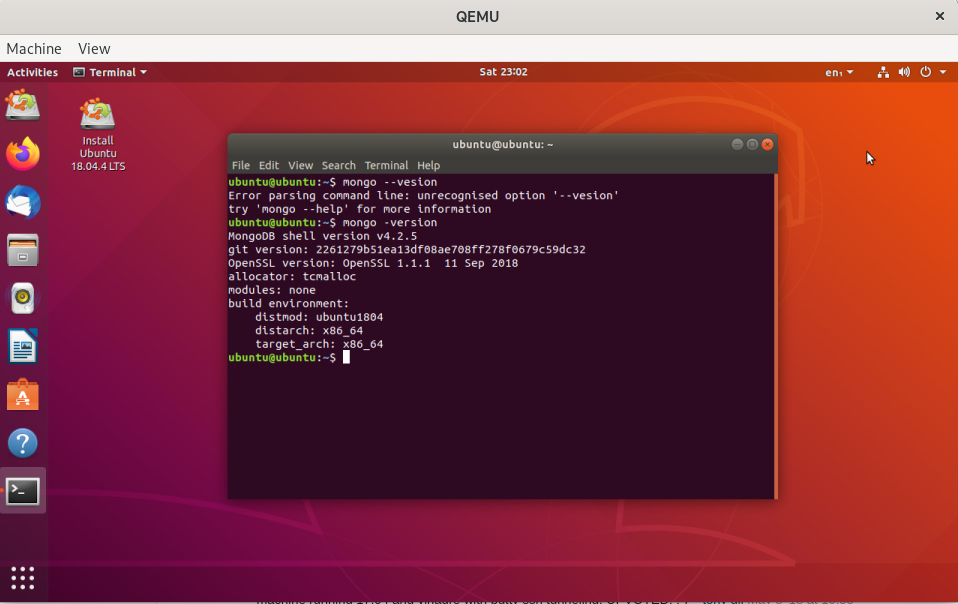
\includegraphics[width=\linewidth]{images/mongoLive.png} 
\newpage
\section*{Modul Java}
\addcontentsline{toc}{section}{\numberline{}Modul Java}
Java je objektno-orijentisani programski jezik opće namjene. Aplikacije napisane u Java programskom jeziku se prije izvršenja kompajliraju u Java bytecode te se izvršavaju u Java virtuelnoj mašini, tako da jedan java program može da se pokrene na bilo kom računaru koji ima instaliran Java Virtual Machine.\\
Java je napravljena od strane Sun Microsystems kompanije te objavljena u maju 1995. godine. Posljednja verzija Java-e je 14, dok je posljednja LTS verzija 11. Postoji nekoliko različitih platformi za koje se distribuira Java, tako da iz toga se mogu definisati 4 grupe Java distribucija:\\
1. Java Card - za kartice\\
2. Java Platform, Micro Edition (ME) - za računare sa ograničenim resursima\\
3. Java Platform, Standard Edition (SE) - za takozvane radne stanice ili "workstations"\\
4. Java Platform, Enterprise Edition (EE) - za velike distribuirane poslovne sisteme i internet okruženja\\
\indent
Slijedi postupak kreiranja Java modula.

\subsection*{Kreiranje direktorija potrebnih za rad}
\addcontentsline{toc}{subsection}{\numberline{}Kreiranje direktorija potrebnih za rad}

\begin{lstlisting}[style=BashInputStyle]
cd ~/squashfs/livecdtmp
sudo mount -o loop ./isoimgs/ubuntu-18.04.4-desktop-amd64.iso mnt
mkdir extract-java-cd
sudo rsync --exclude=/casper/filesystem.squashfs -a mnt/ extract-java-cd
mkdir modul-java
sudo rsync -a extract-java-cd/ modul-java
\end{lstlisting}

\subsection*{unsquashfs filesystem.squashs datoteke}
\addcontentsline{toc}{subsection}{\numberline{}unsquashfs filesystem.squashfs datoteke}

Zatim slijedi korak u kojem se opet raspakuje filesystem.squashfs direktorij i kopiramo ga u edit-java direktorij. Ovaj put ćemo edit direktorij imenovati edit-java da ne izgubimo prethodni sadržaj edit direktorija.\\
\begin{lstlisting}[style=BashInputStyle]
sudo unsquashfs mnt/casper/filesystem.squashfs
sudo mv squashfs-root/ edit-java
\end{lstlisting}
Na slici ispod se vidi output unsquashfs komande:\\
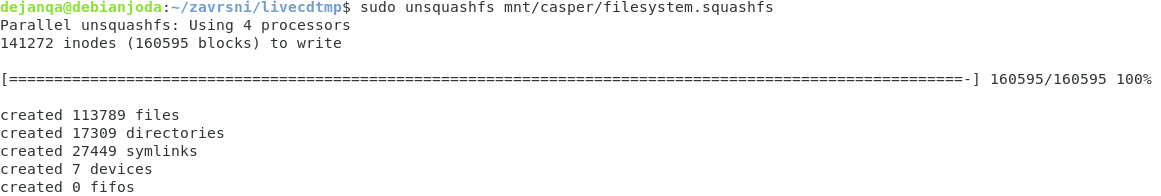
\includegraphics[width=\linewidth]{images/unsquashfscommand.png} 

\subsection*{Konfiguracija paketa za chroot okruženje}
\addcontentsline{toc}{subsection}{\numberline{}Konfiguracija paketa za chroot okruženje}
\noindent
Da bi imali mrežnu konekciju unutar edit-java direktorija jedno rješenje je kopirati /run direktorij unutar edit-java direktorija.
Najbolje manuelno popuniti resolv.conf unutar edit-java direktorija:
\begin{lstlisting}[style=BashInputStyle]
sudo gedit edit-java/etc/resolv.conf
\end{lstlisting}
Te unijeti sljedeći sadržaj i spasiti promjene:
(\textit{nameserver 1.1.1.1 \\
nameserver 8.8.8.8}).\\
\noindent
Isto važi i za etc/hosts datoteku:
\begin{lstlisting}[style=BashInputStyle]
sudo gedit edit-java/etc/hosts
\end{lstlisting}
Kopirati sadrzaj iz /etc/hosts datoteke na sistemu domacinu unutar edit-java/etc/hosts datoteke:
\begin{lstlisting}
127.0.0.1	localhost
127.0.1.1	debianjoda.joda.net	debianjoda
\end{lstlisting}

\noindent
Namjestiti edit-java/dev direktorij kopirajuci /dev/ direktorij sa hosta, zatim chroot u edit-java direktorij.
Obaviti mount instrukcije navedene ispod. Ukoliko korisnik odluči da obriše edit-java direktorij iz nekog razloga,
bilo bi potrebno uraditi unmount edit-java direktorija da sistem domaćin ne bi postao neupotrebljiv:
\begin{lstlisting}[style=BashInputStyle]
sudo mount --bind /dev/ edit-java/dev
sudo chroot edit-java
mount -t proc none /proc
mount -t sysfs none /sys
mount -t devpts none /dev/pts
\end{lstlisting}

\noindent
Takodjer potrebno je izvrsiti sljedece komande da bi se izbjegli problemi sa lokalizacijom:
\begin{lstlisting}[style=BashInputStyle]
export HOME=/root
export LC_ALL=C
\end{lstlisting}

\subsection*{Instalacija Java paketa unutar chroot okruženja}
\addcontentsline{toc}{subsection}{\numberline{}Instalacija Java paketa unutar chroot okruženja}
\noindent
Za ispis svih instaliranih paketa:
\begin{lstlisting}[style=BashInputStyle]
dpkg-query -W --showformat='\${Installed-Size}\t\${Package}\n' | sort -nr | less
\end{lstlisting}

\noindent
Instalacija java paketa:
\begin{lstlisting}[style=BashInputStyle]
apt update
apt install default-jdk
\end{lstlisting}
Provjera verzije java instalacije:
\begin{lstlisting}[style=BashInputStyle]
java -version
\end{lstlisting}
Rezultat prethodne komande bi trebao biti:
\begin{lstlisting}[style=BashInputStyle]
openjdk version "11.0.6" 2020-01-14
OpenJDK Runtime Environment (build 11.0.6+10-post-Ubuntu-1ubuntu118.04.1)
OpenJDK 64-Bit Server VM (build 11.0.6+10-post-Ubuntu-1ubuntu118.04.1, mixed mode, sharing)
\end{lstlisting}
Sada možemo instalirati Eclipse, koji je jedan od najpoznatijih JAVA IDE (Integrated Development Environment). Prvo ćemo preuzeti eclipse.tgz sa interneta pomoću wget komande, a zatim instalirati:
\begin{lstlisting}[style=BashInputStyle]
wget http://ftp.jaist.ac.jp/pub/eclipse/technology/epp/downloads/release/2019-03/R/eclipse-java-2019-03-R-linux-gtk-x86_64.tar.gz
tar -zxvf eclipse-java-2019-*-R-linux-gtk-x86_64.tar.gz -C /usr/
ln -s /usr/eclipse/eclipse /usr/bin/eclipse
nano /usr/share/applications/eclipse.desktop
\end{lstlisting}
Nakon posljednje komande unijeti sljedeći sadržaj:
\begin{lstlisting}[style=BashInputStyle]
[Desktop Entry]
Encoding=UTF-8
Name=Eclipse IDE
Comment=Eclipse IDE
Exec=/usr/bin/eclipse
Icon=/usr/eclipse/icon.xpm
Terminal=false
Type=Application
StartupNotify=false
\end{lstlisting}
Sada možemo pokrenuti eclipse medjutim to ćemo kasnije uraditi kada pokrenemo iso file u kemu-kvm.
\noindent
Nakon završetka instalacije izvršiti unutar chroot:
\begin{lstlisting}[style=BashInputStyle]
apt clean
rm -rf /tmp/* ~/.bash_history
rm -rf /tmp/* ~/.bashrc
rm /var/lib/dbus/machine-id
rm /sbin/initctl
dpkg-divert --rename --remove /sbin/initctl
umount /proc || umount -lf /proc
umount /sys
umount /dev/pts
umount /dev
exit
\end{lstlisting}

\noindent
Ponovno generisati filesystem.manifest:
\begin{lstlisting}[style=BashInputStyle]
sudo chmod +w extract-java-cd/casper/filesystem.manifest
sudo su
chroot edit-java dpkg-query -W --showformat='${Package} ${Version}\n' > extract-java-cd/casper/filesystem.manifest
exit
sudo cp extract-java-cd/casper/filesystem.manifest extract-java-cd/casper/filesystem.manifest-desktop
sudo sed -i '/ubiquity/d' extract-java-cd/casper/filesystem.manifest-desktop
sudo sed -i '/casper/d' extract-java-cd/casper/filesystem.manifest-desktop
\end{lstlisting}

\subsection*{Generisanje filesystem.squashfs direktorija}
\addcontentsline{toc}{subsection}{\numberline{}Generisanje filesystem.squashfs direktorija}
\noindent
Sada cemo upotrijebiti drugu funkciju iz squashfs-tools, a to je mksquashfs. S tom funkcijom ćemo kompresovati edit-java direktorij u novu filesystem.squashfs datoteku, baš kao i u prethodna dva slučaja sa MongoDB i NodeJS modulima. U kodu ispod je potrebno izvršiti komandu iz linije 1 i jednu od preostale 3, pri čemu prva (komanda na liniji 2) daje najslabiju kompresiju, ali je najbrža. Druga komanda se duže izvršava ali je veći procenat kompresije u odnosu na prvu komandu. Dok je kod treće komande procenat kompresije najveći, a vrijeme izvršenja najduže:
\begin{lstlisting}[style=BashInputStyle]
sudo rm extract-java-cd/casper/filesystem.squashfs
sudo mksquashfs edit-java extract-java-cd/casper/filesystem.squashfs -nolzma 
sudo mksquashfs edit-java extract-java-cd/casper/filesystem.squashfs -b 1048576
sudo mksquashfs edit-java extract-java-cd/casper/filesystem.squashfs -comp xz -e edit/boot
\end{lstlisting}

\noindent
Naredni korak je da ažuriramo filesystem.size datoteku:
\begin{lstlisting}[style=BashInputStyle]
sudo su
printf $(du -sx --block-size=1 edit-java | cut -f1) > extract-java-cd/casper/filesystem.size
exit
\end{lstlisting}

\noindent
Nakon toga upisati naziv image-a unutar README.diskdefines. 
Upisati 'Ubuntu with Java 18.04.4 LTS "Bionic Beaver" - Release amd64' u polje DISKNAME:
\begin{lstlisting}[style=BashInputStyle]
sudo gedit extract-java-cd/README.diskdefines
\end{lstlisting}

\subsection*{Generisanje Ubuntu .iso image sa Java modulom}
\addcontentsline{toc}{subsection}{\numberline{}Generisanje Ubuntu .iso image sa Java modulom}
\noindent
Ažurirati md5sum.txt datoteku:
\begin{lstlisting}[style=BashInputStyle]
cd extract-java-cd
sudo rm md5sum.txt
find -type f -print0 | sudo xargs -0 md5sum | grep -v isolinux/boot.cat | sudo tee md5sum.txt
\end{lstlisting}

\noindent
Napokon možemo napraviti iso image koji će da sadrži Java modul. Za ovu operaciju koristimo funkciju genisoimage. Neke linux distribucije nude mkisofs funkciju. Tako da ukoliko ne radi genisoimage trebala bi raditi funkcija mkisofs:
\begin{lstlisting}[style=BashInputStyle]
sudo genisoimage -D -r -V "$IMAGE_NAME" -cache-inodes -J -l -b isolinux/isolinux.bin -c isolinux/boot.cat -no-emul-boot -boot-load-size 4 -boot-info-table -o ../ubuntu-with-java-18.04-amd64.iso .
\end{lstlisting}

\subsection*{Pokretanje iso image-a pomoću kvm biblioteke}
\addcontentsline{toc}{subsection}{\numberline{}Pokretanje iso image-a pomoću kvm biblioteke}
\indent
Sada ćemo napraviti virtuelni hard disk pomocu qemu-img komande da bismo pokrenuli na njemu naš novi modul Java Ubuntu.
\begin{lstlisting}[style=BashInputStyle]
cd ~
qemu-img create ubuntujava.img 5G
\end{lstlisting}

\noindent 
Pokrenućemo modul pomoću KVM-a:
\begin{lstlisting}[style=BashInputStyle]
sudo kvm -hda ubuntujava.img -cdrom ~/zavrsni/livecdtmp/ubuntu-with-java-18.04-amd64.iso -boot d -m 2048
\end{lstlisting}

\subsection*{Rezultat Modul Java}
\addcontentsline{toc}{subsection}{\numberline{}Rezultat Modul Java}
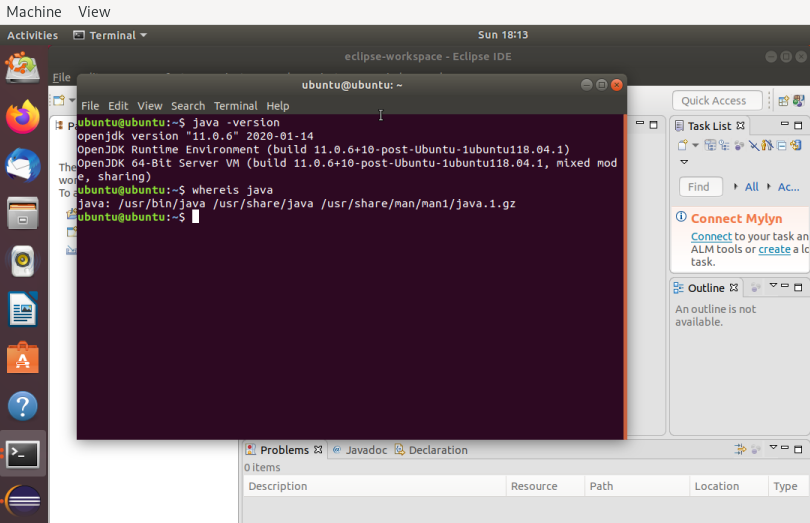
\includegraphics[width=\linewidth]{images/javaLive.png} 
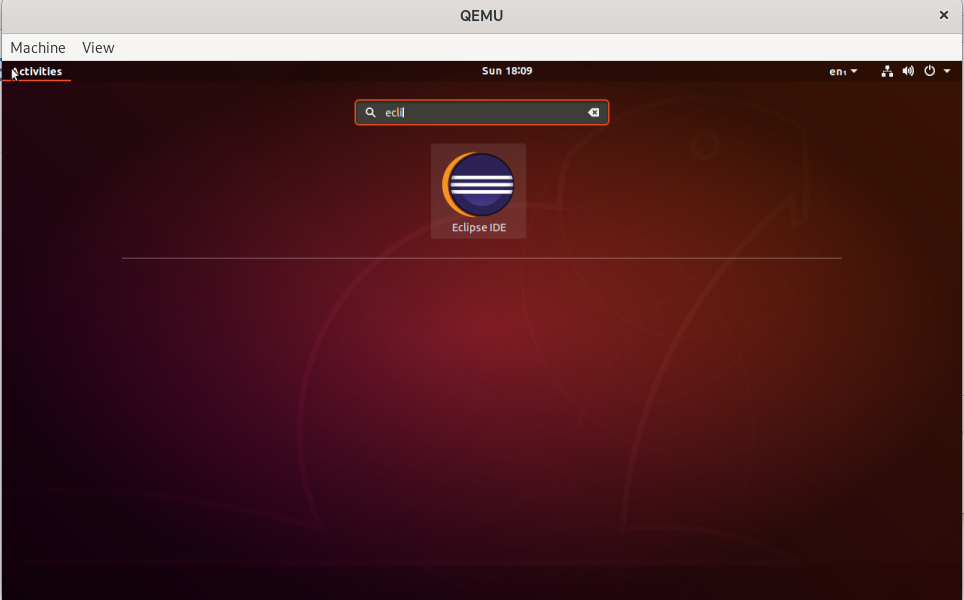
\includegraphics[width=\linewidth]{images/eclipseLive.png} 
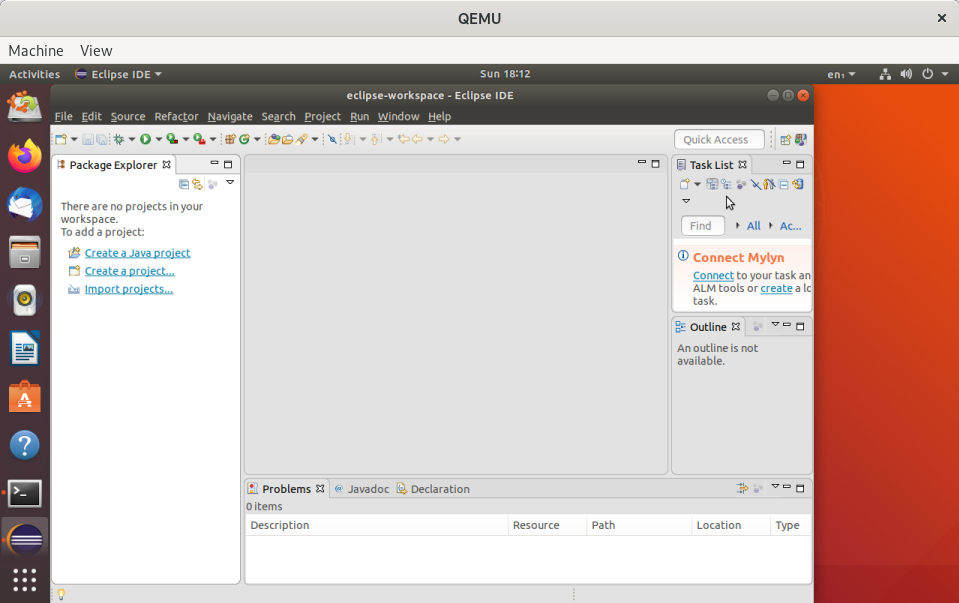
\includegraphics[width=\linewidth]{images/eclipseLive1.png} 
\newpage
\section*{Modul Chrome}
\addcontentsline{toc}{section}{\numberline{}Modul Chrome}
Kao treći primjer modularizacije squashfs datotečnog sistema, kreiran je modul Chrome. Kao što mu ime kaže, riječ je o modulu sa instaliranim Chrome pretraživačem paketima. Većinom koraci su identični kao u prethodna 2 slučaja, izuzev koraka instaliranja dodatnih paketa unutar modula.\\
\subsection*{Kreiranje direktorija potrebnih za rad}
\addcontentsline{toc}{subsection}{\numberline{}Kreiranje direktorija potrebnih za rad}
\begin{lstlisting}[style=BashInputStyle]
cd ~/squashfs/livecdtmp
sudo mount -o loop ./isoimgs/ubuntu-18.04.4-desktop-amd64.iso mnt
mkdir extract-chrome-cd
sudo rsync --exclude=/casper/filesystem.squashfs -a mnt/ extract-chrome-cd
mkdir modul-chrome
sudo rsync -a extract-chrome-cd/ modul-chrome
\end{lstlisting}

\subsection*{unsquashfs filesystem.squashs datoteke}
\addcontentsline{toc}{subsection}{\numberline{}unsquashfs filesystem.squashfs datoteke}

Zatim slijedi korak u kojem se opet raspakuje filesystem.squashfs direktorij i kopiramo ga u edit-chrome direktorij. Ovaj put ćemo edit direktorij imenovati edit-chrome da ne izgubimo prethodni sadržaj edit direktorija.\\
\begin{lstlisting}[style=BashInputStyle]
sudo unsquashfs mnt/casper/filesystem.squashfs
sudo mv squashfs-root/ edit-chrome
\end{lstlisting}

\subsection*{Konfiguracija paketa za chroot okruženje}
\addcontentsline{toc}{subsection}{\numberline{}Konfiguracija paketa za chroot okruženje}
\indent
Da bi imali mrežnu konekciju unutar edit-chrome direktorija jedno rješenje je kopirati /run direktorij unutar edit-chrome direktorija.
Najbolje manuelno popuniti resolv.conf unutar edit-chrome direktorija \\\textit{nameserver 1.1.1.1 \\
nameserver 8.8.8.8}.\\
Isto važi i za etc/hosts datoteku. Najbolje je provjeriti nakon izvršenih komandi da li je upisan sadržaj u resolv.conf i hosts datoteke, te ukoliko nije dopuniti nedostatke:
\begin{lstlisting}[style=BashInputStyle]
sudo cp /etc/resolv.conf edit-chrome/etc/
sudo mount -o bind /run/ edit-chrome/run
\end{lstlisting}

\noindent
Kopirati i hosts direktorij/:
\begin{lstlisting}[style=BashInputStyle]
sudo cp /etc/hosts edit-chrome/etc/
\end{lstlisting}

\noindent
Namjestiti edit-chrome/dev direktorij kopirajući /dev/ direktorij sa hosta, zatim chroot u edit-chrome direktorij.
Obaviti mount instrukcije navedene ispod. Ukoliko korisnik odluči da obriše edit-chrome direktorij iz nekog razloga,
bilo bi potrebno uraditi unmount edit-chrome direktorija da sistem domaćin ne bi postao neupotrebljiv:
\begin{lstlisting}[style=BashInputStyle]
sudo mount --bind /dev/ edit-chrome/dev
sudo chroot edit-chrome
mount -t proc none /proc
mount -t sysfs none /sys
mount -t devpts none /dev/pts
\end{lstlisting}

Također potrebno je izvršiti sljedeće komande da bi se izbjegli problemi sa lokalizacijom:
\begin{lstlisting}[style=BashInputStyle]
export HOME=/root
export LC_ALL=C
\end{lstlisting}

\subsection*{Instalacija Google Chrome paketa unutar chroot okruženja}
\addcontentsline{toc}{subsection}{\numberline{}Instalacija Google Chrome paketa unutar chroot okruženja}
\noindent
Za ispis svih instaliranih paketa:
\begin{lstlisting}[style=BashInputStyle]
dpkg-query -W --showformat='\${Installed-Size}\t\${Package}\n' | sort -nr | less
\end{lstlisting}

\noindent
Instalacija google-chrome paketa:
\begin{lstlisting}[style=BashInputStyle]
sudo nano /etc/apt/sources.list.d/google-chrome.list
\end{lstlisting}
Te upisati u ovu datoteku sljedeći sadržaj
\begin{lstlisting}[style=BashInputStyle]
deb [arch=amd64] http://dl.google.com/linux/chrome/deb/ stable main
\end{lstlisting}
Zatim spasiti datoteku unutar nano editora sa \textbf{CTRL+O}, \textbf{ENTER} za potvrdu i \textbf{CTRL+X} za izlaz iz nano editora.\\
Sljedeća komanda preuzima Google javni ključ da bismo mogli instalirati google-chrome. Zatim komandom apt-key dodajemo ključ u prsten javnih ključeva da bi apt mogao potvrditi integritet Google Chrome paketa.\\
\begin{lstlisting}[style=BashInputStyle]
wget https://dl.google.com/linux/linux_signing_key.pub
sudo apt-key add linux_signing_key.pub
\end{lstlisting}

Sada izvršimo ažuriranje liste paketa i instaliramo google-chrome-stable paket:
\begin{lstlisting}[style=BashInputStyle]
apt update
apt install google-chrome-stable
\end{lstlisting}

Provjera instalacije:
\begin{lstlisting}[style=BashInputStyle]
google-chrome-stable --version
\end{lstlisting}

\noindent
Nakon završetka instalacije izvršiti unutar chroot:
\begin{lstlisting}[style=BashInputStyle]
apt-get clean
rm -rf /tmp/* ~/.bash_history
rm -rf /tmp/* ~/.bashrc
rm /var/lib/dbus/machine-id
rm /sbin/initctl
dpkg-divert --rename --remove /sbin/initctl
umount /proc || umount -lf /proc
umount /sys
umount /dev/pts
exit
\end{lstlisting}

\noindent
Ponovno generisati filesystem.manifest:
\begin{lstlisting}[style=BashInputStyle]
sudo chmod +w extract-chrome-cd/casper/filesystem.manifest
sudo su
chroot edit-chrome dpkg-query -W --showformat='${Package} ${Version}\n' > extract-chrome-cd/casper/filesystem.manifest
exit
sudo cp extract-chrome-cd/casper/filesystem.manifest extract-chrome-cd/casper/filesystem.manifest-desktop
sudo sed -i '/ubiquity/d' extract-chrome-cd/casper/filesystem.manifest-desktop
sudo sed -i '/casper/d' extract-chrome-cd/casper/filesystem.manifest-desktop
sudo umount edit/dev
\end{lstlisting}

\subsection*{Generisanje filesystem.squashfs direktorija}
\addcontentsline{toc}{subsection}{\numberline{}Generisanje filesystem.squashfs direktorija}
\noindent
Sada cemo upotrijebiti drugu funkciju iz squashfs-tools, a to je mksquashfs. S tom funkcijom cemo kompresovati edit-chrome direktorij u novu filesystem.squashfs datoteku. U kodu ispod je potrebno izvršiti komandu iz linije 1 i jednu od preostale 3, pri čemu prva (komanda na liniji 2) daje najslabiju kompresiju, ali je najbrza. Druga komanda se duže izvršava ali je veći procenat kompresije u odnosu na prvu komandu. Dok je kod treće komande procenat kompresije najveći, a vrijeme izvršenja najduže:
\begin{lstlisting}[style=BashInputStyle]
sudo rm extract-chrome-cd/casper/filesystem.squashfs
sudo mksquashfs edit-chrome extract-chrome-cd/casper/filesystem.squashfs -nolzma 
sudo mksquashfs edit-chrome extract-chrome-cd/casper/filesystem.squashfs -b 1048576
sudo mksquashfs edit-chrome extract-chrome-cd/casper/filesystem.squashfs -comp xz -e edit/boot
\end{lstlisting}

\noindent
Naredni korak je da ažuriramo filesystem.size datoteku:
\begin{lstlisting}[style=BashInputStyle]
sudo su
printf $(du -sx --block-size=1 edit-mysql | cut -f1) > extract-chrome-cd/casper/filesystem.size
exit
\end{lstlisting}

\noindent
Nakon toga upisati naziv image-a unutar README.diskdefines. 
Upisati 'Ubuntu with Google Chrome 18.04.4 LTS "Bionic Beaver" - Release amd64' u polje DISKNAME:
\begin{lstlisting}[style=BashInputStyle]
sudo gedit extract-chrome-cd/README.diskdefines
\end{lstlisting}

\subsection*{Generisanje Ubuntu .iso image sa Google Chrome modulom}
\addcontentsline{toc}{subsection}{\numberline{}Generisanje Ubuntu .iso image sa Google Chrome modulom}
\noindent
Ažurirati md5sum.txt datoteku:
\begin{lstlisting}[style=BashInputStyle]
cd extract-chrome-cd
sudo rm md5sum.txt
find -type f -print0 | sudo xargs -0 md5sum | grep -v isolinux/boot.cat | sudo tee md5sum.txt
\end{lstlisting}

\noindent
Napokon možemo napraviti iso image koji će da sadrži Google Chrome modul. Za ovu operaciju koristimo funkciju genisoimage. Neke linux distribucije nude mkisofs funkciju. Tako da ukoliko ne radi genisoimage trebala bi raditi funkcija mkisofs:
\begin{lstlisting}[style=BashInputStyle]
sudo genisoimage -D -r -V "$IMAGE_NAME" -cache-inodes -J -l -b isolinux/isolinux.bin -c isolinux/boot.cat -no-emul-boot -boot-load-size 4 -boot-info-table -o ../ubuntu-with-chrome-18.04-amd64.iso .
\end{lstlisting}

\subsection*{Pokretanje iso image-a pomoću kvm biblioteke}
\addcontentsline{toc}{subsection}{\numberline{}Pokretanje iso image-a pomoću kvm biblioteke}
\indent
Sada ćemo napraviti virtuelni hard disk pomocu qemu-img komande da bismo pokrenuli na njemu naš novi modul Google Chrome Ubuntu.
\begin{lstlisting}[style=BashInputStyle]
cd ~
qemu-img create ubuntuchrome.img 5G
\end{lstlisting}

\noindent 
Pokrenucemo modul pomoću KVM-a:
\begin{lstlisting}[style=BashInputStyle]
sudo kvm -hda ubuntuchrome.img -cdrom ~/zavrsni/livecdtmp/ubuntu-with-chrome-18.04-amd64.iso -boot d -m 2048
\end{lstlisting}

\subsection*{Rezultat Modul Chrome}
\addcontentsline{toc}{subsection}{\numberline{}Rezultat Modul Chrome}
\indent
Ovje će biti tekst + slike vezano za GoogleChrom Modul.
%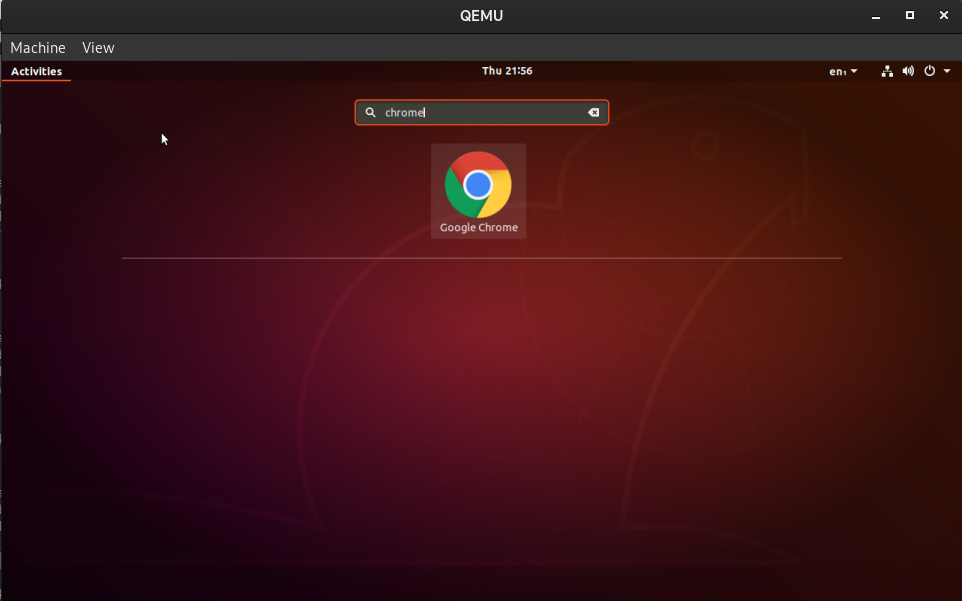
\includegraphics[width=\linewidth]{images/chromeLive.png} 


\end{document}
